\chapter{Introduction}

\section{Contexte}

Dans le cadre de ma 4\up{ème} année d'étude à Polytech Grenoble en informatique, j'ai effectué mon stage de 12 semaines à Universiti Teknologi PETRONAS (UTP) à Seri Iskandar, en Malaisie. Ce stage s'est déroulé du \textbf{20 mai 2019} au \textbf{9 août 2013}.

À l'occasion de la mise en place d'un futur parternariat entre Polytech Grenoble et UTP, différents sujet de stage ont été transmis aux étudiants de Polytech par le bureau des relations internationnales. Au final, nous étions 4 étudiants : j'ai été accompagné de 2 autres étudiants venant de la spécialité INFO (Informatique) et 1 étudiants de IESE (Informatique et Electronique des Systèmes Embarqués).


\begin{figure}[h]
  \centering
  \begin{subfigure}{.5\textwidth}
    \centering
    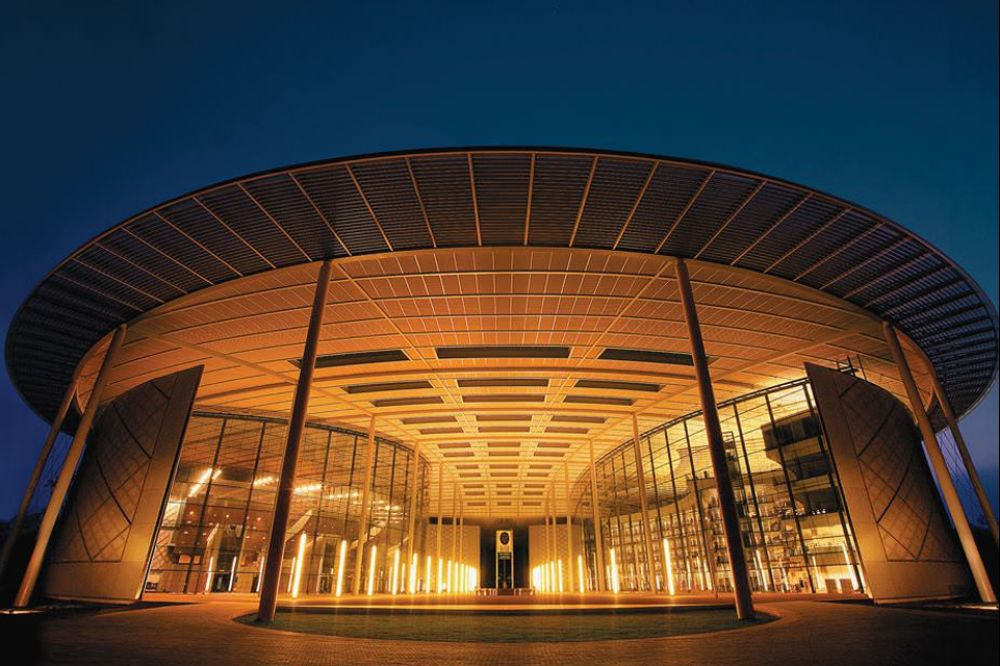
\includegraphics[width=.8\linewidth]{content/imgs/utp.jpg}
    \caption{Bibliothèque de l'université}
  \end{subfigure}%
  \begin{subfigure}{.5\textwidth}
    \centering
    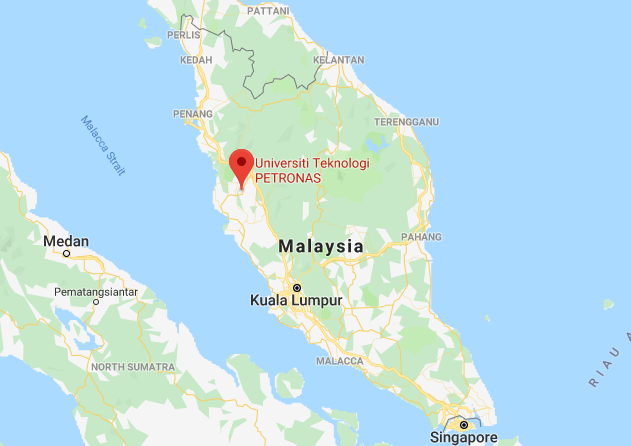
\includegraphics[width=.8\linewidth]{content/imgs/map.png}
    \caption{UTP, Seri Iskandar, Malaisie}
  \end{subfigure}
  \caption{Universiti Teknologi PETRONAS}
\end{figure}




\section{Sujet proposé}

Le sujet proposé à pour objectif de developper une application mobile dans le but d'aider les personnes atteintent de baiegement à surpasser ce trouble de la parole.

Une application similaire a déjà été développer durant 3 années par des étudiants dans le cadre de leurs \textit{Final year project}. Comme illustré dans l'annexe \ref{appendix:old_app}, cette application propose les fonctionnalités suivantes :

\begin{itemize}
  \item Des exercices pour apprendre à controler son flux de parole ;
  \item La possibilité de visualiser sa progression pour chaque exercices ;
  \item Des informations concernant le bégaiement.
\end{itemize}

Cette application était disponible sur les appareils Android via le Play Store, la plateforme de téléchargement d'application developpé par Google. Suite à un trop grand nombre de retours de bug concernant l'application, celle-ci a dû être retiré du Play Store.

Le sujet qui m'a été proposé est de recommencer dépuis le début le developpement de cette application, en reprenant donc les fonctionnalités précédemment présentés.

Dans sa version finale, l'application devra donc proposée différents exercices pour apprendre à controler son flux de parole ainsi que la possibilité de visualiser sa progression pour chacun des exercices accompagné de graphique illustrant la progression de l'utilisateur. De plus, l'application pourra être utiliser par des orthophonistes pour accéder à la progression de leurs patients. Ils pourront aussi donner des retours et des commentaires.

Aucune autre contrainte (technologies, organisations, etc.) m'a été imposé.


\section{But du rapport}
Ce rapport est destiné à tous ceux qui souhaite avoir un aperçu global du projet et de ce qui a été réalisé durant ces 12 semaines. En particulier, ce rapport est un bon point d'entrée pour tous ceux qui souhaite continuer le developpement de \textit{Stuttherapy}. Le rapport est disponible en version anglaise et française.

\section{Organisation du rapport}

La rapport est tout d'abort constitué de cette partie, l'introduction où j'ai présenter le contexte dans lequelle le stage a été effectué et où j'ai donner une description succinte du sujet proposé.

Ensuite, la deuxième partie décrit le travail effectivement réalisé lors de ce stage, notamment tout le processus de reflexion, de recherches, de conception, d'organisation, de developpement, de tests et finalement de production.

La troisième partie est consacrée aux connaissances que j'ai acquise et améliorées durant ces 12 semaines. Je reviendrais sur les erreurs que j'ai commises, leurs causes, leurs conséquences.

Avant de conclure ce rapport, une page sera consacrée au developpement durable, en vertu de la loi Grenelle 1 de 2009 sur l'environnement.





















%
